\chapter{DMDTE}
%\section{Cosa è un Digital Twin}
%Un \textit{digital twin} - in italiano \textit{gemello digitale} - è la copia digitale di un oggetto fisico e reale, sia questo oggetto ancora nella fase di progettazione, fase di prototipazione, fase di validazione, o in fase di uso operativo.
%\medbreak
%\
%Affinché un digital twin si possa considerare tale, quindi non più strettamente coincidere con la simulazione di un sistema o model, il gemello digitale deve essere in qualche \textit{relazione con l'ambiente reale}.
%\medbreak
%Definiamo allora come \textit{real twin} la controparte fisica e reale del \textit{digital twin}, \textit{digital model} un model totalmente digitale della controparte fisica, e come \textit{thread} - \textit{filo} in italiano - il flusso di dati bidirezionale tra i due gemelli.
%\medbreak
%Distinguiamo anche l'ambiente operativo di real twin e digital model:
%\begin{itemize}
%	\item Il \textbf{real twin} ha come ambiente di lavoro il \textbf{mondo reale}, pertanto percepisce questo per mezzo di \textit{sensori}, e a sua volta interagisce su di esso per mezzo di \textit{attuatori}.
%	\item Il \textbf{digital model} ha come ambiente di lavoro un \textbf{mondo virtuale}, il quale deve essere quanto più fedele possibile nel rappresentare la sua controparte reale, tuttavia non precludendo la possibilità di possedere \textit{informazioni aggiuntive}, come oggetti puramente virtuali, o anche semplificazioni di modelli cinematici e dinamici; il digital twin interagisce con l'ambiente virtuale mediante gli strumenti messi a disposizione dal software in cui questo è sviluppato, i quali potrebbero anche essere a loro volta digital twin di sensori o attuatori reali; infine, in quanto questo sia un mondo digitale, non vi è incertezza d'informazione, pertanto è possibile interrogare il sistema mondo e ottenere informazioni esatte su di esso e le entità che lo popolano.
%\end{itemize}
%
%Allora, possiamo definire il \textbf{digital twin} quando vi è uno scambio di dati, un \textit{thread} o \textit{filo} tra le due entità, quindi un digital twin è una entità che \textbf{interagisce con} e \textbf{percepisce} entrambi i mondi, \textbf{reale} e \textbf{digitiale}.
%
%\subsection{Livelli di integrazione}
%Le definizioni date fino ad ora, sono basate sul lavoro svolto da Werner Kritzinger et al. \cite{KRITZINGER20181016}, il quale articolo si presenta come una analisi categorica della letteratura scientifica sui digital twin fino all'anno 2018, formalizzando il concetto di digital twin secondo le sue relazioni con l'ambiente reale.
%
%In particolare, tale lavoro si propone come punto di incontro tra le varie definizioni di digital twin, andando ad individuare tre sottocategorie di gemelli digitali come mostrato in Figura. \ref{fig:dt_data_integration}, differenziandole in base al flusso di dati scambiati tra i due gemelli, in particolare vengono suddivisi in \textit{digital model}, \textit{digital shadow} e \textit{digital twin}.
%
%\begin{itemize}
%	\item Un \textbf{digital model} è un model digitale di un oggetto, esso può essere messo in relazione con l'ambiente reale, e quindi il gemello reale, tuttavia ciò non è necessario o richiesto, lo scambio è manuale.
%	\item Un \textbf{digital shadow} è un digital model che riceve dati dall'ambiente esterno per mezzo del gemello reale, tuttavia non è necessario che questo interagisca con l'ambiente reale.
%	\item Un \textbf{digital twin} è quindi un digital shadow che scambia attivamente dati con l'ambiente reale per mezzo del gemello reale, pertanto interagisce attivamente con l'ambiente reale e risponde ad esso.
%\end{itemize}
%
%Come già accennato, è ruolo del \textit{thread} mettere in comunicazione il gemello reale e il gemello digitale. 
%\begin{figure}[htbp]
%  \centering
%  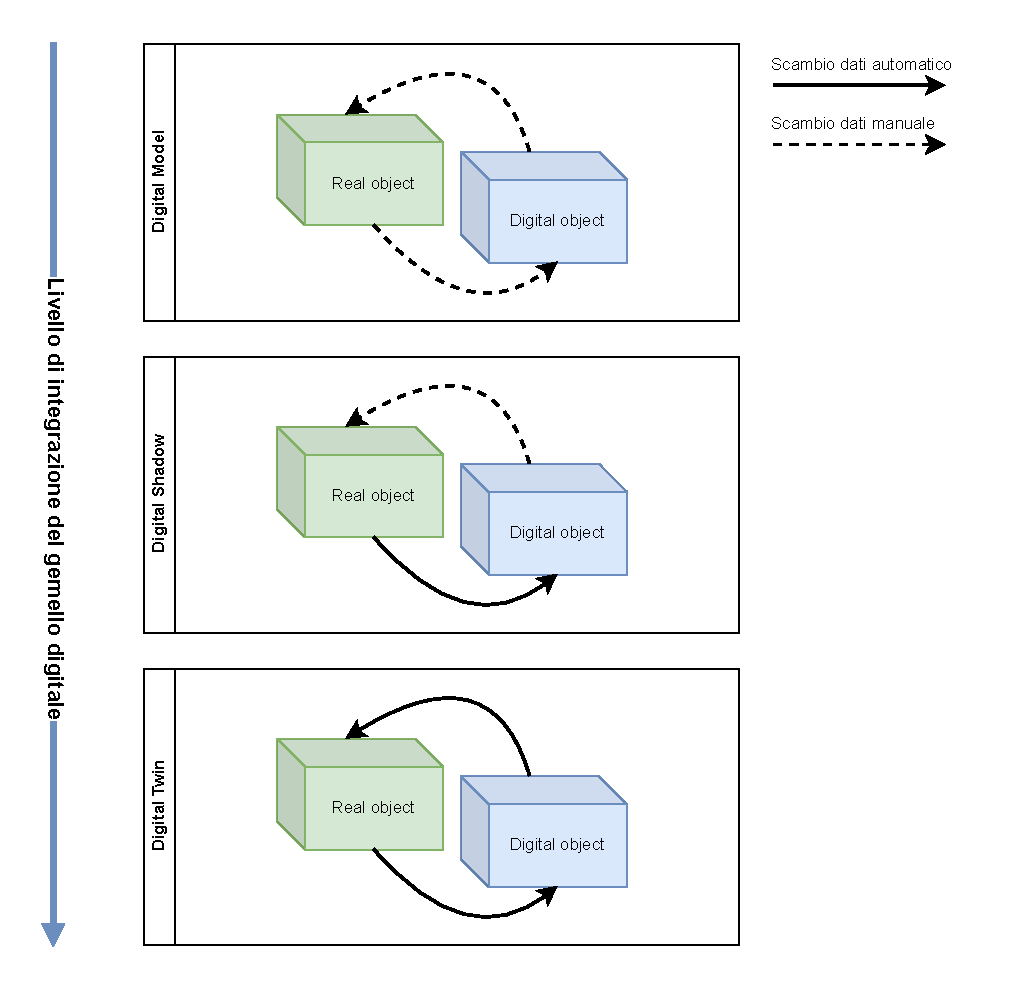
\includegraphics[width=1.0\textwidth, page=1]{Images/cristo.pdf}
%  \caption{Livelli di integrazione dati nei digital twin.}
%  \label{fig:dt_data_integration}
%\end{figure}
%
%
%\subsection{Origine}
%Non è possibile andare ad individuare una origine ben precisa dell'idea del digital twin, in quanto si può considerare una convergenza di idee, infatti noi umani studiamo ambiente e oggetti circostanti, creandone una rappresentazione mentale per mezzo dei nostri organi sensoriali, processi cognitivi e conoscenza, con tale rappresentazione dunque riconosciamo ambienti per navigare con più sicurezza, riconosciamo e usiamo oggetti con padronza: pertanto trasporre questo nostro processo intrinseco in ambito computazionale non è che una conseguenza del fatto che questo processo, naturale e trasparente per noi, sia una idea vincente da applicare per sistemi artificiali più intelligenti, sicuri e affidabili.
%\medbreak
%Una prima formalizzazione in letteratura viene da uno studio sul \textit{Product lifecycle management} PLM - in italiano \textit{gestione del ciclo di vita di un prodotto} - nel 2005 da Grieves \cite{grieves2005}, nel suo studio sul ciclo di vita di un prodotto - ideazione, produzione, operatività e smaltimento - considera fondamentale l'informazione, introduce pertanto il concetto di \textbf{Mirrored Space Models}, un model che consiste dei tre elementi che caratterizzano  anche l'idea moderna del digital twin: oggetto fisico, model virtuale e scambio di dati tra loro.
%\medbreak
%
%La nascita del termine vero e proprio di digital twin lo sì deve alla NASA in ambiente aerospaziale, in particolare in \textit{The digital twin paradigm for future NASA and U.S. air force vehicles (2012)} \cite{nasa2012} viene introdotto il digital twin come un complesso e ultra realistico model simulativo del veicolo reale, il quale usa i migliori modelli fisici disponibili, sia integrato con i sistemi e sensori del veicolo e sia esattamente speculare al veicolo stesso. L'obiettivo del digital twin secondo NASA è quello di salvaguardiare ulteriormente lo stato di salute del veicolo quando questo è in missione, fornendone un model digitare per il monitoraggio del veicolo, correzione degli errori, mitigazione danni e eventi non prevedibili etc. attività non immediatamente correggibili o prevedibili in fase di progettazione e produzione nonostante le migliori tecnologie, dunque per la seconda volta l'idea di base di digital twin si propone come strumento fondamentale per il ciclo di vita di un prodotto (il veicolo spaziale).
%\medbreak
%
%Dal 2016 in poi, con l'evoluzione tecnologica, l'introduzione massiva dell'Internet Of Things, la necessità dell'integrazione digitale nell'industria e nei prodotti di uso comune, la nascita dell'industria 4.0 con la sua esigenza di integrare il digitale con la produzione e il ciclo di vita dei prodotti, si osserva un significativo aumento della letteratura scientifica sugli studi relativi ai digital twin, correlata a una confusione generale del termine, specie nella sua relazione con \textit{digital model} e \textit{digital shadow}, come documentato da Werner Kritzinger et al. \cite{KRITZINGER20181016} e da \textit{Digital Twin: Origin to Future (2021)} \cite{origin2021}, cui definisce il digital twin come:
%
%\begin{quote}
%\textit{Un Digital Twin è un model o una simulazione digitale/virtuale, dinamica e capace di auto-evolversi, di un soggetto o oggetto reale (componente, macchina, processo, essere umano, ecc.), che rappresenta lo stato esatto del suo gemello fisico in ogni istante tramite lo scambio di dati in tempo reale e la conservazione dei dati storici. Non è solo il Digital Twin a imitare il suo gemello fisico: anche qualsiasi variazione nel Digital Twin viene imitata dal gemello fisico.}
%\end{quote}
%
%\pagebreak
\parbox{1.0\textwidth}{
	\textbf{Distributed Multi Agent Digital Twin Environment} (DMDTE) è una \textit{architettura} per la progettazione di complessi sistemi multi-agente Digital Twin.
}
\medskip

Al fine di comprendere la sua implementazione, è necessario spiegare il suo modello generale.

Consideriamo, in ordine, un modello più semplice singola a istanza e singolo gemello digitale al fine di chiarere i concetti di base, successivamente viene introdotto il modello più generale distribuito e multi istanza.
\pagebreak
\begin{figure}[ht]
  \centering
	\includegraphics[page=2, width=1.0\textwidth]{Images/cristo.pdf}
	\caption{Modello singolo agente: in basso l'ambiente reale e le sue entità, in alto ambiente virtuale con le sue entità, tra esse digital twin di entità reali.}
  \label{fig:dmdte-single-instance}
\end{figure}
\section{Modello singolo agente}
\parbox{1.0\textwidth}{
	Il modello singolo agente fornisce un ottimo punto di partenza per la descrizione di un sistema digital twin ad agenti, possiamo trovare una sua rappresentazione grafica nella \autoref{fig:dmdte-single-instance}, la quale illustra un semplice sistema digital twin a singolo agente.
	}
\medbreak


Bisogna distinguere due ambienti: 
l'\textbf{ambiente reale}, posto nella parte inferiore della figura, contiene le entità reali del mondo reale, nel caso di esempio un peluche e un robot; l'\textbf{ambiente virtuale}, posto nella parte superiore della figura, è una copia virtuale dell'ambiente reale, del quale ne emula topologia e proprietà fisica, ed è popolato da \textit{digital twin} e \textit{virtual agent}.

L'\textbf{ambiente virtuale} è interamente simulato da un software, nella implementazione presentata \textit{Godot}, in esso vi possiamo trovare:
\begin{itemize}
	\item Il \textbf{digital twin} di un agente robotico reale in esempio un Alvik.
	\item Il \textbf{digital twin} di un oggetto o ostacolo reale, in esempio un peluche di \textit{capybara}.
	\item \textbf{Agenti virtuali} e \textbf{ostacoli virtuali}, in esempio un agente robotico virtuale, un ostacolo a forma di cono stradale e un ostacolo a forma di parallelepipedo.
\end{itemize}

Come si può notare dalla figura, gli oggetti reali hanno una corrispondenza digitale: il \textit{digital twin}. Oggetti statici come il peluche di capybara possono essere rappresentati staticamente nel mondo virtuale con approssimate geometrie, sufficienti a rappresentarne una presenza nello spazio come ostacolo.
\medskip

Gli \textbf{agenti robotici} o dinamici, analogamente agli ostacoli, possiedono un \textit{digital twin}, dotato di uno flusso bidirezionale e automatico di informazioni per mezzo di un \textit{collegamento} fra il \textit{real twin} e \textit{digital twin} \cite{KRITZINGER20181016}. Nel contesto del DMDTE il real agent deve possedere una unità di calcolo sufficiente per eseguire la \textbf{Real Agent Interface}, una API che esponga le funzionalità e lo stato dell'agente stesso.
\medbreak

Il \textit{Real Agent Interface} comunica per mezzo del \textbf{Digital Twin Protocol}, in breve DTP, con la sua controparte digitale. Il DTP è un protocollo di comunicazione realizzato per DMDTE, il suo scopo è quello di permettere la sincronizzazione di stato tra agente reale e gemello digitale e l'invocazione di metodi per mezzo di \textit{chiamate a procedura remota}.
Nel contesto di DTP, identifichiamo come peer DTP un gemello reale o virtuale, e come DTP host l'applicazione che ospita gemelli digitali e permette la loro comunicazione con il loro reale.
\medbreak

Il \textit{digital twin} dell'agente robotico, infine, è una entità composta da due oggetti: il \textit{model} dell'agente robotico, in grado di interagire con l'ambiente virtuale, e il \textit{ghost}. Il ghost è sincronizzato in tempo reale per mezzo di DTP con l'agente reale, tuttavia come un fantasma, non è in grado di interagire con l'ambiente virtuale. Il model è potenzialmente in grado di interagire con l'ambiente virtuale, deve essere dotato di un modello tridimensionale, dinamiche fisiche, e deve interagire con l'ambiente virtuale in modi quanto più simili a come il gemello reale interagisce con l'ambiente reale. 
\medbreak

Ghost e model sono sempre tenuti in \textit{stretta vicinanza} e corrispondenza di posa, inoltre le simulazioni fisiche avvenute nel model digitale, successivamente alla loro esecuzione, si ripercuotono nel gemello reale tramite DTP, il cui a sua volta risponderà di conseguenza riportando il suo stato successivo al \textit{ghost}, andando così a costruire un sistema di feedback automatico.
\medbreak

Assegnando dei \textbf{controller} al model, ovvero programmi o script che definiscono uno specifico comportamento e controllo definiti dal programmatore in Godot, è possibile specificare un comportamento ben preciso per il digital twin: è allora possibile definire un controller che segua un determinato percorso, sia questo definito da una logica dettata da sensori di prossimità, line follower o da un \textit{navigation agent} di Godot, oppure permettere a un utente umano il controllo del robot: controllando il \textit{model}, viene a sua volta coinvolto il \textit{real twin}, e di conseguenza aggiornato il \textit{ghost}, creando un ciclo di feedback automatico; pertanto si identifica il sistema \textit{ghost/model} come gemello digitale.
\medbreak

Infine è possibile anche definire \textbf{agenti completamente virtuali}, ovvero entità dinamiche del mondo virtuale che non hanno corrispondenza reale, controllabili con gli stessi \textit{controller} definiti per il \textit{digital twin/model}, tali agenti possono essere utili per effettuare pure simulazioni, esplorare ambienti, aggiungere ostacoli dinamici, oppure rappresentare all'interno dell'ambiente virtuale entità reali la quale tuttavia si ha un alto grado di incertezza relativa sul loro stato, come per esempio entità catturate da un sistema di computer vision.
\medbreak


\begin{figure}[t]
  \centering
	\includegraphics[page=3, width=1.0\textwidth]{Images/cristo.pdf}
  %\includegraphics[width=1.0\textwidth]{Images/distributed-multi-agent.drawio.pdf}
  \caption{Modello del sistema multi agente e distribuito}
  \label{fig:dmdte}
\end{figure}
\section{Modello multi agente distribuito}
Definito il modello a singolo agente semplice, consideriamo lo scenario in cui più agenti robotici e più istanze di mondi virtuali debbano coesistere e coordinarsi tra loro.
\medbreak

Senza perdere di generalità, consideriamo il caso di due agenti digital twin e tre istanze di ambiente virtuale, tale architettura è esemplificata dalla Figura \ref{fig:dmdte}.
\medbreak

Come mostrato in figura, ognuno degli agenti robotici è collegato per mezzo di DTP a una istanza esclusiva di Godot, una terza istanza di Godot funge da osservatore: ogni istanza è in comunicazione con le altre per mezzo della \textbf{MultiplayerAPI}, un insieme di strumenti e API che permettono la creazione di un ambiente virtuale replicato tra istanze di rete integrato in Godot, la quale in modo trasparente al programmatore si occupa della sincronizzazione dello stato delle entità presenti nella scena, dell'ambiente virtuale e la gestione di eventuali comunicazioni per mezzo di \textit{chiamata a procedura remota}. Nel contesto della \textit{MultiplayerAPI}, la singola istanza di Godot prende il nome di \textbf{multiplayer peer}. Un peer multiplayer può anche essere un \textit{DTP host} e ospitare più istanze di \textit{digital twin}, in tal caso identifichiamo come \textit{autorità} l'istanza di \textit{multiplayer peer} che ospita un determinato \textit{digital twin} e il suo DTP peer; una istanza può non ospitare alcun gemello virtuale o non essere DTP host e comportarsi da semplice osservatore.
\medbreak

Con questo modello, le istanze di ambiente virtuale e agenti digitali sono replicati e sincronizzati, permettendo una integrazione trasparente di unità di calcolo eterogenee in grado di collaborare tra loro per coordinare gli agenti.
\medbreak

Gemelli digitali anche di diverse istanze allora possono collaborare tra loro per compiere task in modo coordinato.
